%%%%% --------------------------------------------------------------------------------
%%
%%                           Document Template of NUDT proposal
%%
%%%%% --------------------------------------------------------------------------------
%% Copyright (C) Hanlin Tan <hanlin_tan@nudt.edu.cn> 
%% This is free software: you can redistribute it and/or modify it
%% under the terms of the GNU General Public License as published by
%% the Free Software Foundation, either version 3 of the License, or
%% (at your option) any later version.
%%%%% --------------------------------------------------------------------------------
%% Last Updated: 2017.01.06
%%%%************************ Document Class Declaration ******************************
%%
%\documentclass{ctexart}

\documentclass{Style/nudtproposal}% thesis template of UCAS
%% Multiple optional arguments:
%% [scheme = plain] % for thesis writing of international students
%% [<singlesided|doublesided|printcopy>] % single-sided, double-sided, or print layout
%% [draftversion] % show draft version information, default is no show
%% [fontset = <adobe|...>] % specify font set, default is automatic detection
%% [standard options for ctex class]
%%%%% --------------------------------------------------------------------------------
%%
%%%%************************* Command Define and Settings ****************************
%%
\usepackage{Style/commons}% common settings
%% usage: \usepackage[option1,option2,...,optionN]{commons}
%% Multiple optional arguments:
%% [myhdr] % one available header and footer style, will enable fancyhdr
%% [lscape] % provide landscape layout environment
%% [geometry] % configure page layout by geometry package
%% [list] % enable enhanced list environments, useful for Algorithm and Coding
%% [color] % enable color package to use color, default package is xcolor
%% [background] % enable page background, will auto enable color package
%% [tikz] % enable tikz for complex diagrams, will auto enbale color package
%% [table] % enable a table package for complex tables, default is ctable
%% [math] % enable some extra math packages
\usepackage{Style/custom}% user defined commands

%% 正文需要的宏
\usepackage{mdframed} % 页面边框
\usepackage{titlesec}   %设置页眉页脚的宏包
\usepackage{fancyhdr} % 页眉页脚
\usepackage{tabularx}  % 表格宽度
\usepackage{multirow} % 表格单元格合并
\usepackage{caption}   % 图表标题
% demo new tabular bibliography format
\usepackage{csquotes}
\usepackage[american]{babel}
%\usepackage[backend=biber, bibstyle=numeric, citestyle=numeric]{biblatex} % 设定引用格式
%\usepackage[backend=biber, style=caspervector,utf8, sorting=nty]{biblatex} % 设定引用格式
%\usepackage[backend=biber, style=Biblio/nudtcaspervector,utf8, sorting=none]{biblatex} % 设定引用格式
%\usepackage[backend=biber, style=gbt77142005, utf8]{biblatex} % 设定引用格式
\usepackage{longtable}


% 重定义图表标题
%\renewcommand{\figurename}{图 } 
%\renewcommand{\tablename}{表 } 
\captionsetup[figure]{labelfont={},name={图 },labelsep=space}
\captionsetup[table]{labelfont={},name={表 },labelsep=space}

% 重定义标题格式
%\titleformat{command}[shape]{format}{label}{sep}{before-code}{after-code}
\titleformat{\section}{\heiti}{\thesection、}{5 pt}{}
\titlespacing*{\section} {0pt}{0ex}{.2ex} % 设置标题前后间距
\titleformat{\subsection}{\kaishu \small \bfseries}{\thesubsection}{5 pt}{}
\titleformat{\subsubsection}{\kaishu \small}{\thesubsubsection}{5 pt}{}
% 定义upcite
\newcommand{\upcite}[1]{\textsuperscript{ [\cite{#1}]  }} % 中文引用
%\newcommand{\upcite}[6]{\textsuperscript{ [\cite{#1,#2,#3,#4,#5,#6}] }} % 中文引用

\newcommand{\tabincell}[2]{\begin{tabular}{@{}#1@{}}#2\end{tabular}} % 单元格换行
% 首页图案
\schoollogo{scale=0.35}{nudt_logo}% university logo
\schooltext{scale=0.9}{nudt_text}% university logo

% 定义字符串比较函数
\makeatletter
\def\instring#1#2{TT\fi\begingroup
	\edef\x{\endgroup\noexpand\in@{#1}{#2}}\x\ifin@}
\makeatother


% 修改参考文献格式
% 开题报告类型
\newcommand\enabletablebib[1]{%	
	\ifstrequal{#1}{yes}{\newcommand\printbib{\printbibtabular[title={~}]}	}{	\newcommand\printbib{\printbibliography[title={~}]}}
}



\makeatletter
% user-level command for printing tabular bibliography
\let\printbibtabular\printbibliography
\patchcmd{\printbibtabular}{\blx@printbibliography}{\bbx@printbibtabular}{}{}
\patchcmd{\printbibtabular}{\blx@printbibliography}{\bbx@printbibtabular}{}{}

\let\bbx@printbibtabular\blx@printbibliography
\patchcmd{\bbx@printbibtabular}{\blx@bibliography}{\bbx@bibtabular}{}{}
\patchcmd{\bbx@printbibtabular}
{\def\blx@theenv{bibliography}}{\def\blx@theenv{bibtabular}}{}{}

% underlying macros
\def\bbx@bibtabular#1{%
	\blx@bibheading\blx@theheading\blx@thetitle
	\blx@bibnote\blx@theprenote
	\begingroup
	\blx@bibinit
	\let\@noitemerr\@empty
	\let\blx@noitem\blx@warn@bibempty
	\ifnum\bibinitsep=\z@
	\let\blx@initsep\relax
	\fi
	\ifnum\bibnamesep=\z@
	\let\blx@namesep\relax
	\fi
	\csuse{blx@hook@bibinit}%
	% copy filtered list of entries to internal list macro
	\def\blx@do##1{%
		\blx@ifdata{##1}{%
			\begingroup
			\blx@getdata{##1}
			\blx@bibcheck
			\iftoggle{blx@skipentry}{}{%
				\global\let\blx@noitem\@empty
				\listadd\blx@tempa{##1}}%
			\endgroup}{}}
	\let\blx@done\relax
	
	% 文献计数器
	\newcounter{count}
	\value{count}=0 % 初值为0
	\blx@listloop{#1}
	% tabular output for each item in list macro 表格中的每行内容(& 为分隔符, \\ \hline 为换行和横线)
	%	\def\do##1{\bbx@tab@label{##1} & \bbx@tab@item{##1} \\ \hline}
	\def\do##1{ \stepcounter{count}  % count++
		[\arabic{count}] & \bbx@tab@item{##1} \\ \hline  %表格一行的内容
	}
	\csuse{blx@env@\blx@theenv}%
	\dolistloop{\blx@tempa}
	\csuse{blx@endenv@\blx@theenv}%
	\blx@bibnote\blx@thepostnote
	\endgroup}

\def\bbx@tab@label#1{%
	\begingroup
	\blx@getdata{#1}%
	\blx@setoptions@type\abx@field@entrytype
	\blx@setoptions@entry
	\blx@thelabelnumber
	\blx@addprefixnumber
	\addtocounter{instcount}\@ne
	\csuse{bbx@tabenv@\blx@theenv}\relax
	\endgroup}

\def\bbx@tab@item#1{% 定义每行参考文献的具体内容
	\begingroup
	\blx@getdata{#1}%
	\blx@setoptions@type\abx@field@entrytype
	\blx@setoptions@entry
	\csuse{blx@item@\blx@theenv}\relax
	\blx@initsep
	\blx@namesep
	\csuse{blx@hook@bibitem}%
	\blx@execute
	\blx@initunit
	%	\blx@anchor %此参数会造成额外空行
	\blx@beglang
	\bibsentence
	\blx@pagetracker
	\blx@driver\abx@field@entrytype
	\blx@postpunct
	\blx@endlang
	\endgroup}

% user-level command for defining tabular bibliography format
\newrobustcmd*{\defbibtabular}[5]{%
	\long\csdef{blx@env@#1}{#2}%
	\long\csdef{blx@endenv@#1}{#3}%
	\long\csdef{bbx@tabenv@#1}{#4}%
	\long\csdef{blx@item@#1}{#5}}

% user-level access to some entry options
\def\useeditorfalse{\togglefalse{blx@useeditor}}
\def\usetranslatorfalse{\togglefalse{blx@usetranslator}}

\makeatother

% sortname labels (a robust style should add provision for missing labelnames)
\newbibmacro*{sortname}{% 表格第一列内容
	\renewcommand*{\multinamedelim}{\addslash\break}%
	\let\finalnamedelim\multinamedelim
	\printtext[plain]{\printnames[last-first]{labelname}}}
%    \printfield{number}}

% bibitem hook to suppress redundant sortname list   % hook 表格第二列内容
\newbibmacro*{omitsortname}{%
	\ifnameundef{labelname}{}{%
		\ifnameundef{author}
		{\ifnameundef{editor}
			{\ifusetranslator{\clearname{translator}}{}}}
		{\clearname{editor}}
		{\clearname{author}}%
		\useeditorfalse%
		\usetranslatorfalse}}

% demo new tabular bibliography format
\defbibtabular{bibtabular}
{\noindent
	\begin{longtable}{| p{0.10\textwidth} < {\centering}| p{0.85\textwidth}|  }
		\hline
		{\songti 序号}  & \multicolumn{1}{c|}{\songti 文献目录(作者、题目、刊物名、出版时间、页次)} \\
		\hline
	}
	{  \hline \end{longtable}  \indent }
{\usebibmacro{sortname}}
{\usebibmacro{omitsortname}}

%\bibliographystyle{Biblio/gbt-7714-2015-numerical}
%\addbibresource{Biblio/ref.bib}
\newcommand{\cmd}[1]{\texttt{\textbackslash #1}}
 % 包含作者自定义的格式和命令
%%%%% ---------------------------------------------------------------------------------
%%%%% ---------------警告:以上内容请勿随意修改,除非你清楚自己在做什么------------


%%%%% --------------提示:修改本节内容用于设置文档,请仔细阅读---------------------
%% 
%% 编译环境:texlive-2015。
%% 推荐IDE:texstudio(WinXXX 太挫了)。
%% 编译选项:tex编译器选择xelatex, 参考文献编译器选择biber(不能用bibtex)!
%% 以上环境配置经过作者测试,确定可以正常使用。

%%%%% ---------------提示:本参数提供一个参考文献格式BUG的临时解决方案------------
% 是否将参考文献放入表格。这个选项的设置因为参考文献格式有一个暂时无解的BUG。设置为yes之前之前,必须先
% 设置为no编译一次。否则正文中引用数字都是0。
% 最终提交前将此参数改为yes编译一次。注意:设置为yes后编译第二次就会出现正文中引用数字都是0的BUG!
% 如果设置为yes后,还需要修改正文,那么改为no,编译  两次 参考文献才会正常!
\enabletablebib{no}   % 最终提交前将此参数改为yes编译一次! 如需修改正文,改为no后编译两次参考文献才会正常!   

%% 以下参数用于设置文档首页和页眉信息
\proposaltype{doctor}          % 研究生类别:硕士设置为master,博士设置为doctor 
\enabletableofcontents{no}   % 是否生成目录:如果需要目录设置为yes,否则设置为no。我校开题报告默认没有目录
\proposalnumber{\underline{\hbox to 10mm{}}}          % 编号:默认是下划线,如果你知道编号,设为真实编号
\classification{公开}              % 密级:公开,秘密,机密或者绝密
\nudttitle{国防科学技术大学开题报告}{\LaTeX{} 模板} % 因title一般都很长需要两行,第一参数为第一行内容,第二个参数为第二行内容
\author{谭同学}                    % 作者
\authorid{160590xx}            % 学号
\advisor{张老师}                   % 导师
\advisortitle{教~~~~授}         % 职称
\degreetype{工学}                 % 学位类别
\major{控制科学与工程}          % 一级学科
\field{图像处理}                      % 研究方向
\institute{信息系统与管理学院}% 学院
\chinesedate{2017~年~03~月~01日} % 开题日期
\formdate{二零一七年三月}     % 制表月份 注意:用“〇”可能会出现字体不显示的问题,所以这里改为了“零”

%% 在设置完以上参数后,修改Tex文件下对应文件以完成开题报告。
%%%%% ---------------------------------------------------------------


%%%%% ---------------警告:以下内容请勿随意修改,除非你清楚自己在做什么------------

%%%%******************************** Content *****************************************
%%
\begin{document}
%%
%%%%% --------------------------------------------------------------------------------
%%
%%%%******************************** Frontmatter *************************************
%%
\pagenumbering{roman}% restart page numbers with arabic style
%%% Generate Title
%%
\maketitle

%%%%% --------------------------------------------------------------------------------
%%
%%%%******************************** Mainmatter **************************************
%%

%% 添加正文内容
\pagenumbering{arabic}% restart page numbers with arabic style
\mdfsetup{skipabove=0pt,skipbelow=0pt}
%% 包含正文各个章节,请编辑章节文件修改相应的内容
%%%%% --------------------------------------------------------------------------------
%%
%%%%******************************* Main Content *************************************
%%
%%% ++++++++++++++++++++++++++++++++++++++++++++++++++++++++++++++++++++++++++++++++++




\section{文献学位论文选题的立论依据}


\begin{mdframed}[everyline=true]
	
\subsection{课题来源}
自拟。


\subsection{基本概念}
\subsubsection{异常事件}
异常,新华词典的解释是“不同于平常”\upcite{a6-1}。从分类的角度看,异常与正常是两个大类别,异常内部又可以分成打架、撞车等小类别。从概率的角度看\upcite{1-4},“平常”是大多数,而“异常”就是少数,所以异常事件,则可解释为“小概率事件”。
    异常事件的分类有很多角度。根据场景运动目标的多少,可以分为拥挤场景的异常事件和不拥挤场景的异常事件。这种分类主要根据基于跟踪和轨迹分析的异常检测方法能否适用。拥挤场景现有的跟踪方法都会失效,而不拥挤场景基于跟踪和轨迹分析的方法是可能奏效的。根据异常事件的规模,可以分为全局异常事件(如图 1)和局部异常事件(如图 2)。这种分类可以用于决定异常警报的级别。根据异常事件是基于先验知识还是场景学习,可以分为特定类型异常事件和广义异常事件\upcite{biblatex}。

%% ----------------注意: mdframed 中不能使用 figure 和 table。用以下示例方法替代。----------------
\begin{center}
	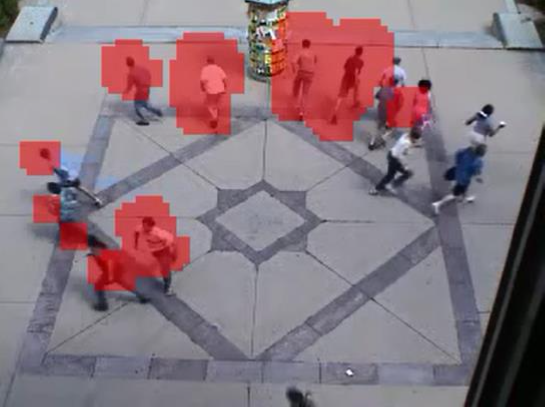
\includegraphics[width=0.7\linewidth]{Img/fig1}
	\captionof{figure}{人群四散逃离的异常事件(全局异常事件)} % \caption{} 改为 \captionof{figure}{}
	\label{fig:fig1}
\end{center}

\begin{center}
	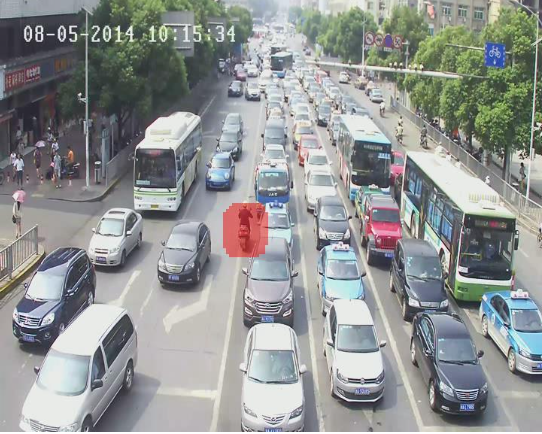
\includegraphics[width=0.7\linewidth]{Img/fig2}
	\captionof{figure}{摩托车违章逆行的异常事件(局部异常事件)} % \caption{} 改为 \captionof{figure}{}
	\label{fig:fig2}
\end{center}


\begin{center}
	\captionof{table}{一张表}   % \caption{} 改为 \captionof{table}{}
	\begin{tabular}{lrrr} \hline
		年份        & 乡村 & 城市 & 所有   \\ \hline
		1983        & 38.7  & 55.6  & 44.7  \\
		1993–1994   & 50.3  & 66.4  & 54.3  \\
		2004–2005   & 50.2  & 69.3  & 55    \\
		2009–2010   & 51.7  & 71.6  & 57.1  \\ \hline
		\multicolumn{4}{@{}l@{}}{\footnotesize 来源: http://tomheaven.cn} 
	\end{tabular}
    \label{tab:tab1}
\end{center}

\subsubsection{广义异常事件}

本课题认为从分类的角度检测到的是特定类型异常事件\upcite{2-5_2},而从概率的角度检测到的是广义异常事件\upcite{li2000}。例如打架斗殴、人群逃散、交通事故都是根据人们的先验知识确定的异常事件,在绝大多数场景中,只要发生这样的事件,就肯定是异常事件。而广义异常事件与特定类型异常事件相对,是指不能由人们的先验知识预先设定类别,而是由监控视频场景决定的异常事件。发生概率低和与场景相关是广义异常事件的本质特征。

例如图 2的摩托车逆行,只有发生在此场景的城市道路上,才是异常事件。如果发生在了无人烟的乡村土路上并不算是异常。而摩托车是不是逆行,也只有放在此特定的场景中才能判断。

\subsection{研究意义}
    随着视频监控在商场、银行、小区、道路等公共场所的广泛部署\upcite{Cong2011Sparse},监控视频数据大量产生。目前监控视频主要还是用于威慑犯罪和事后调取,但视频智能分析的需要一直存在。近期发生了一些引起公众关注的事件再次体现了监控视频异常检测需求的迫切性。IBM深圳公司的一名女经理在地铁口突发心脏病跌倒,虽然正对着监控,却因为监控无人查看而耽误了抢救时间,最终不幸去世。对于这种紧急情况,仅有八分钟的黄金抢救时间,不能及时发现险情和施救生命就会逝去。
    监控视频的异常检测在安防领域、交通管理、城市管理方面有广阔的应用前景。从监控视频中自动发打架斗殴、交通违章、交通事故、人群聚集等事件具有及时发现事故险情,提前发现安全隐患的作用。例如图 3中的行人违规横穿马路,说明此路段存在交通安全隐患,有必要派出交警或者增设警示标志。如果这种情况持续发生,可以考虑架设人行天桥来引导行人。而这种安全隐患靠人工是很难发现和统计的。

  随着计算能力的不断进步,满足视频智能分析需求的计算成本在不断降低,视频智能分析的技术也在不断进步,为监控视频智能分析的普及准备着技术条件,智能监控的时代正在迫近。异常事件检测,作为视频智能分析的重要一环,能够帮助及早发现安全隐患,对异常事件实时发出警报,对于利用监控视频保障安全、处置险情,有重要作用。 
\\[8 cm]
\end{mdframed}

%%% ++++++++++++++++++++++++++++++++++++++++++++++++++++++++++++++++++++++++++++++++++
%   \include ?= \input + \clearpage
\clearpage
%%%%% --------------------------------------------------------------------------------
%%
%%%%******************************* Main Content *************************************
%%
%%% ++++++++++++++++++++++++++++++++++++++++++++++++++++++++++++++++++++++++++++++++++




\section{文献综述}
\begin{mdframed}[everyline=true]
	
   很多文献……  
  \\[20 cm]
\end{mdframed}



%%% ++++++++++++++++++++++++++++++++++++++++++++++++++++++++++++++++++++++++++++++++++
%
\clearpage
%%%%% --------------------------------------------------------------------------------
%%
%%%%******************************* Main Content *************************************
%%
%%% ++++++++++++++++++++++++++++++++++++++++++++++++++++++++++++++++++++++++++++++++++




\section{研究内容}
\begin{mdframed}[everyline=true]
	
\subsection{主要研究内容及拟解决的相关科学问题和技术问题}
	
\subsection{拟采取的研究方法、技术路线、实施方案及可行性分析}

\subsection{预期研究成果和创新点}

很多内容……
\\[10 cm]
\end{mdframed}


%%% ++++++++++++++++++++++++++++++++++++++++++++++++++++++++++++++++++++++++++++++++++
%
\clearpage
%%%%% --------------------------------------------------------------------------------
%%
%%%%******************************* Main Content *************************************
%%
%%% ++++++++++++++++++++++++++++++++++++++++++++++++++++++++++++++++++++++++++++++++++




\section{研究条件}
\begin{mdframed}[everyline=true]

{\bfseries \kaishu \zihao{5} 开展研究应具备的条件及已具备的条件,可能遇到的困难与问题和解决措施。}
\\[20 cm]
\end{mdframed}

%%% ++++++++++++++++++++++++++++++++++++++++++++++++++++++++++++++++++++++++++++++++++
%
\clearpage
%%%%% --------------------------------------------------------------------------------
%%
%%%%******************************* Main Content *************************************
%%
%%% ++++++++++++++++++++++++++++++++++++++++++++++++++++++++++++++++++++++++++++++++++




\section{学位论文工作计划}
{
\noindent
\begin{tabular*}{0.999\textwidth}{| p{0.07\textwidth } <{\centering} | p{0.45\textwidth}  | p{0.162\textwidth} | p{0.20\textwidth}  |}

	\hline 
	序号 & 	\multicolumn{1}{c}{主要研究内容} & 	\multicolumn{1}{|c}{起讫日期} & 	\multicolumn{1}{|c|}{预期成果} \\
	\hline 
	1  &  内容 &  \tabincell{c}{2017年01月 \\至 \\2017年12月} & 很多论文 \\ 
	\hline 
	2   &  &  &  \\ 
	\hline 
	3    &  &  &  \\ 
	\hline 
	4    &  &  &  \\ 
	\hline 
	5    &  &  &  \\ 
	\hline 
\end{tabular*} 
\indent
}


%%% ++++++++++++++++++++++++++++++++++++++++++++++++++++++++++++++++++++++++++++++++++
%
\clearpage

%%%%% --------------------------------------------------------------------------------
%%
%%%%******************************* Main Content *************************************
%%
%%% ++++++++++++++++++++++++++++++++++++++++++++++++++++++++++++++++++++++++++++++++++


\section{主要参考文献}
\printbib
%\printbibtabular[title={~}]
%\printbibliography[title={~}]

%%% ++++++++++++++++++++++++++++++++++++++++++++++++++++++++++++++++++++++++++++++++++
%
\clearpage
%%%%% --------------------------------------------------------------------------------
%%
%%%%******************************* Main Content *************************************
%%
%%% ++++++++++++++++++++++++++++++++++++++++++++++++++++++++++++++++++++++++++++++++++




\section{指导教师对开题报告的评语}
\begin{mdframed}[everyline=true]
   \indent
   
   论文选题源自应用中的实际需求,针对监控视频中的异常事件检测方法开展研究,对 视频智能监控领域和在视频监控实际应用都具有重要意义。
   
   报告对监控视频异常检测方法的国内现状种进行了综述,指出目前有两类主要方法: 对异常视频序列建模的方法和对正常视频序列建模的方法,并对后者更为具体的方法、模 型进行了详细阐述。参阅的论文范围合理,代表性强,为论文研究进一步开展并提出新方 法奠定了基础。
   
   报告提出的两个研究内容针对监控视频异常事件监测中的两个关键环节,拟采取的研 究方法合理、技术路线清晰,初步试验结果表明报告提出方法的可行性。
论文开展研究需要的基础条件具备,对可能遇到的困难与问题有清楚的认识并有对应 的解决措施。论文研究计划合理,参考文献格式规范。
\\[8 cm]
\end{mdframed}

%%% ++++++++++++++++++++++++++++++++++++++++++++++++++++++++++++++++++++++++++++++++++
%
\clearpage
%%%%% --------------------------------------------------------------------------------
%%
%%%%******************************* Main Content *************************************
%%
%%% ++++++++++++++++++++++++++++++++++++++++++++++++++++++++++++++++++++++++++++++++++


\section{开题报告评议小组意见及评议结果}
\begin{mdframed}[everyline=true]

\begin{enumerate}[label={(\arabic*)},labelsep= 3 pt]
	\item {\songti 选题依据、研究内容、研究方案及技术路线的科学性、可行性及创新性的评价}
	
	\quad\quad  谭XX同学的硕士学位论文深入分析国内外的理论观点和技术方案,对监控视频异常事 件检测思路比较清晰,研究方法具有创新性,选题具有重要的应用价值。论文研究内容与工 作量适合硕士学位论文的要求,论文研究方法可行。
	经评议小组讨论,一致同意谭XX同学的硕士学位论文开题报告。
	
	\item  {\songti 存在的主要问题和修改建议 }
	\begin{enumerate}[label={\arabic*)},labelsep=3 pt]
		\item 论文不必提出“广义异常事件”的概念,只需说明工作内容为异常事件检测而不是区分 异常事件的具体类别。
		\item 异常事件检测如果不限定应用场景范围难度和工作量较大,建议先设定一个具体的场景 以降低难度,逐步推进。
		\item 光流的导数(加速度)也可以作为特征向量的一个维度。
		\item 如果采用的方法是无监督的可能更具有实用性。
	\end{enumerate}

	\item  {\songti 开题报告评议结果}
	
    $\square$  {\songti 通过} \quad\quad \quad \quad  $\square$ {\songti 不通过,且要求在2个月内重新组织开题}
	\\[20pt]
	
	
	{  \songti
	\quad\quad\quad\quad \quad\quad\quad\quad 	\quad\quad\quad\quad \quad\quad\quad\quad 组长(签名):
	
	\quad\quad\quad\quad \quad\quad\quad\quad 	\quad\quad\quad\quad \quad\quad\quad\quad \quad\quad\quad 年  \quad\quad 月  \quad\quad 日
	\\
    }
\end{enumerate}
\end{mdframed}
\vspace{-4pt}
{
	\noindent
\begin{tabular*}{0.999\textwidth}{| c  | c | c | p{0.5\textwidth}< {\centering} | p{0.157\textwidth}<{\centering}|}
%	\hline 
    \multicolumn{5}{|c|}{	\songti 开题报告评议小组组成}	\\
	\hline
	{\songti 组成} & {\songti 姓名} & {\songti 职称} &  {\songti  所在单位} & {\songti 本人签名}  \\
	\hline 
	{\songti 组长}     &  张老师 & 教授 &  五院XXXX研究所 &  \\ 
	\hline 
	\multirow{4}{8pt}{\songti 成员}  & 李老师  &  教授&  五院XXXX研究所 & \\ 
	\cline{2-5}
	   &  王老师 &  教授&  X院XXXX研究所 & \\ 
	\cline {2-5}
	   &  谭老师 &  教授&  五院XXXX研究所 & \\ 
	\cline {2-5}
	   &  老老师 &  教授&  五院XXXXXX系 & \\ 
	\hline 
	{\songti 秘书}   & 赖老师 & 讲师 &  五院XXXXXX系 & \\ 
	\hline 
\end{tabular*} 
   \indent
}


%%% ++++++++++++++++++++++++++++++++++++++++++++++++++++++++++++++++++++++++++++++++++
%
\clearpage

\end{document}
%%%%% --------------------------------------------------------------------------------
